\chapter{Interpolation and approximation}%
\label{cha:interpolation_and_approximation}

\minitoc

\section*{Introduction}
In this chapter,
we study numerical methods for interpolating and approximating functions.
The Cambridge dictionary defines interpolation as \emph{the addition of something different in the middle of a text, piece of music, etc.~or the thing that is added}.
The concept of interpolation in mathematics is consistent with this definition;
interpolation consists in finding, given a set of points~$(x_i, y_i)$,
a function~$f$ in a finite-dimensional space that goes through these points.
Throughout this course, you have used the~\julia{plot} function in Julia,
which performs piecewise linear interpolation for drawing functions,
but there are a number of other standard interpolation methods.
Our first goal in this chapter is to present an overview of these methods and the associated error estimates.

In the second part of this chapter,
we focus of \emph{function approximation},
which is closely related to the subject of mathematical interpolation.
Indeed, a simple manner for approximating a general function by another one in a finite-dimensional space is to select a set of real numbers on the $x$ axis,
called \emph{nodes}, and find the associated interpolant.
As we shall demonstrate, not all sets of interpolation nodes are equal,
and special care is required in order to avoid undesired oscillations.
The field of function approximation is vast,
so our aim in this chapter is to present only an introduction to the subject.
In order to quantify the quality of an approximation,
a metric on the space of functions,
or a subset thereof, must be specified in order to measure errors.
Without a metric, saying that two functions are close is almost meaningless!
% Consider, for example, the function $f\colon [0, 1] \to \real; x \mapsto 0$ and the approximations $\widehat f_1(x) = x^{100}$ and $\widehat f_2(x) = 0.01$

\section{Function interpolation}
Assume that we are given $n+1$ nodes $x_0, \dotsc, x_n$ on the $x$ axis,
together with the values $u_0, \dotsc, u_n$ taken by an unknown function~$u(x)$ when evaluated at these points,
and suppose that we are looking for an interpolation~$\widehat u(x)$ in a subspace~$\Span \{\varphi_0, \dotsc, \varphi_n\}$
of the space of continuous functions, i.e.~an interpolating function of the form
\[
    \widehat u(x) = \alpha_0 \varphi_0(x) + \dotsb + \alpha_n \varphi_n(x),
\]
where $\alpha_0, \dotsc, \alpha_n$ are real coefficients.
In order for~$\widehat u(x)$ to be an interpolating function,
we must require that
\[
    \forall i \in \{0, \dotsc, n\}, \qquad
    \widehat u(x_i) = u_i.
\]
This leads to a linear system of $n+1$ equations and $n+1$ unknowns,
the latter being the coefficients~$\alpha_0, \dotsc, \alpha_n$.
This system of equations in matrix form reads
\begin{equation}
    \label{eq:linear_system_interpolation}
    \begin{pmatrix}
        \varphi_0(x_0) & \varphi_1(x_0) & \hdots & \varphi_n(x_0) \\
        \varphi_0(x_1) & \varphi_1(x_1) & \hdots & \varphi_n(x_1) \\
        \vdots & \vdots & & \vdots \\
        \varphi_0(x_n) & \varphi_1(x_n) & \hdots & \varphi_n(x_n)
    \end{pmatrix}
    \begin{pmatrix}
        \alpha_0 \\
        \alpha_1 \\
        \vdots \\
        \alpha_n
    \end{pmatrix}
    =
    \begin{pmatrix}
        u_0 \\
        u_1 \\
        \vdots \\
        u_n
    \end{pmatrix}.
\end{equation}

\subsection{Vandermonde matrix}
Since polynomials are very convenient for evaluation, integration, and differentiation,
they are a natural choice for interpolation purposes.
The simplest basis of the subspace of polynomials of degree less than or equal to $n$ is given by the monomials:
\[
    \varphi_0(x) = 1,
    \qquad
    \varphi_1(x) = x,
    \qquad \dotsc, \qquad
    \varphi_n(x) = x^n.
\]
In this case,
the linear system~\eqref{eq:linear_system_interpolation} for determining the coefficients of the interpolant reads
\begin{equation}
    \label{eq:linear_system_interpolation_poly}
    \begin{pmatrix}
        1 & x_0 & \hdots & x_0^n \\
        1 & x_1 & \hdots & x_1^n \\
        \vdots & \vdots & & \vdots \\
        1 & x_n & \hdots & x_n^n
    \end{pmatrix}
    \begin{pmatrix}
        \alpha_0 \\
        \alpha_1 \\
        \vdots \\
        \alpha_n
    \end{pmatrix}
    =
    \begin{pmatrix}
        u_0 \\
        u_1 \\
        \vdots \\
        u_n
    \end{pmatrix}.
\end{equation}
The matrix on the left-hand side is called a \emph{Vandermonde} matrix.
If the abcissae $x_0, \dotsc, x_n$ are distinct,
then this is a full rank matrix,
and so~\eqref{eq:linear_system_interpolation_poly} admits a unique solution,
implying as a corollary that the interpolating polynomial exists and is unique.
It is possible to show that the condition number of the Vandermonde increases dramatically with $n$,
and so solving~\eqref{eq:linear_system_interpolation_poly} is not a viable method in practice for calculating the interpolating polynomial.

\subsection{Lagrange interpolation formula}
One may wonder whether polynomial basis functions $\varphi_0, \dotsc, \varphi_n$ can be defined in such a manner that
the matrix in~\eqref{eq:linear_system_interpolation} is the identity matrix.
The answer to this question is positive;
it suffices to take as a basis the \emph{Lagrange polynomials},
which are given by
\[
    \varphi_{i}(x)
    = \frac{(x - x_0) (x - x_1) \dotsc (x - x_{i-1}) (x - x_{i+1}) \dotsc (x - x_n)}
    {(x_i - x_0) (x_i - x_1) \dotsc (x_i - x_{i-1}) (x_i - x_{i+1}) \dotsc (x_i - x_n)}.
\]
It is simple to check that
\[
    \varphi_i(x_j) =
    \delta_{i,j} =
    \begin{cases}
        1 & \text{if $i = j$}, \\
        0 & \text{otherwise.}
    \end{cases}
\]
Finding the interpolant in this basis is immediate:
\[
    \widehat u(x) = u_1 \varphi_1(x) + \dotsb + u_n \varphi_n(x).
\]
While simple, this approach to polynomial interpolation has a couple of disadvantages:
first, evaluating $\widehat u(x)$ is computationally costly when $n$ is large and,
second, all the basis functions change when adding new interpolation nodes.
In addition, Lagrange interpolation is numerically unstable because of cancellations between large terms.
Indeed, it is often the case that Lagrange polynomials take very large values over the interpolation intervals;
this occurs, for example,
when many equidistant interpolation nodes are employed,
as illustrated in~\cref{fig:lagrange}.
\begin{figure}[ht]
    \centering
    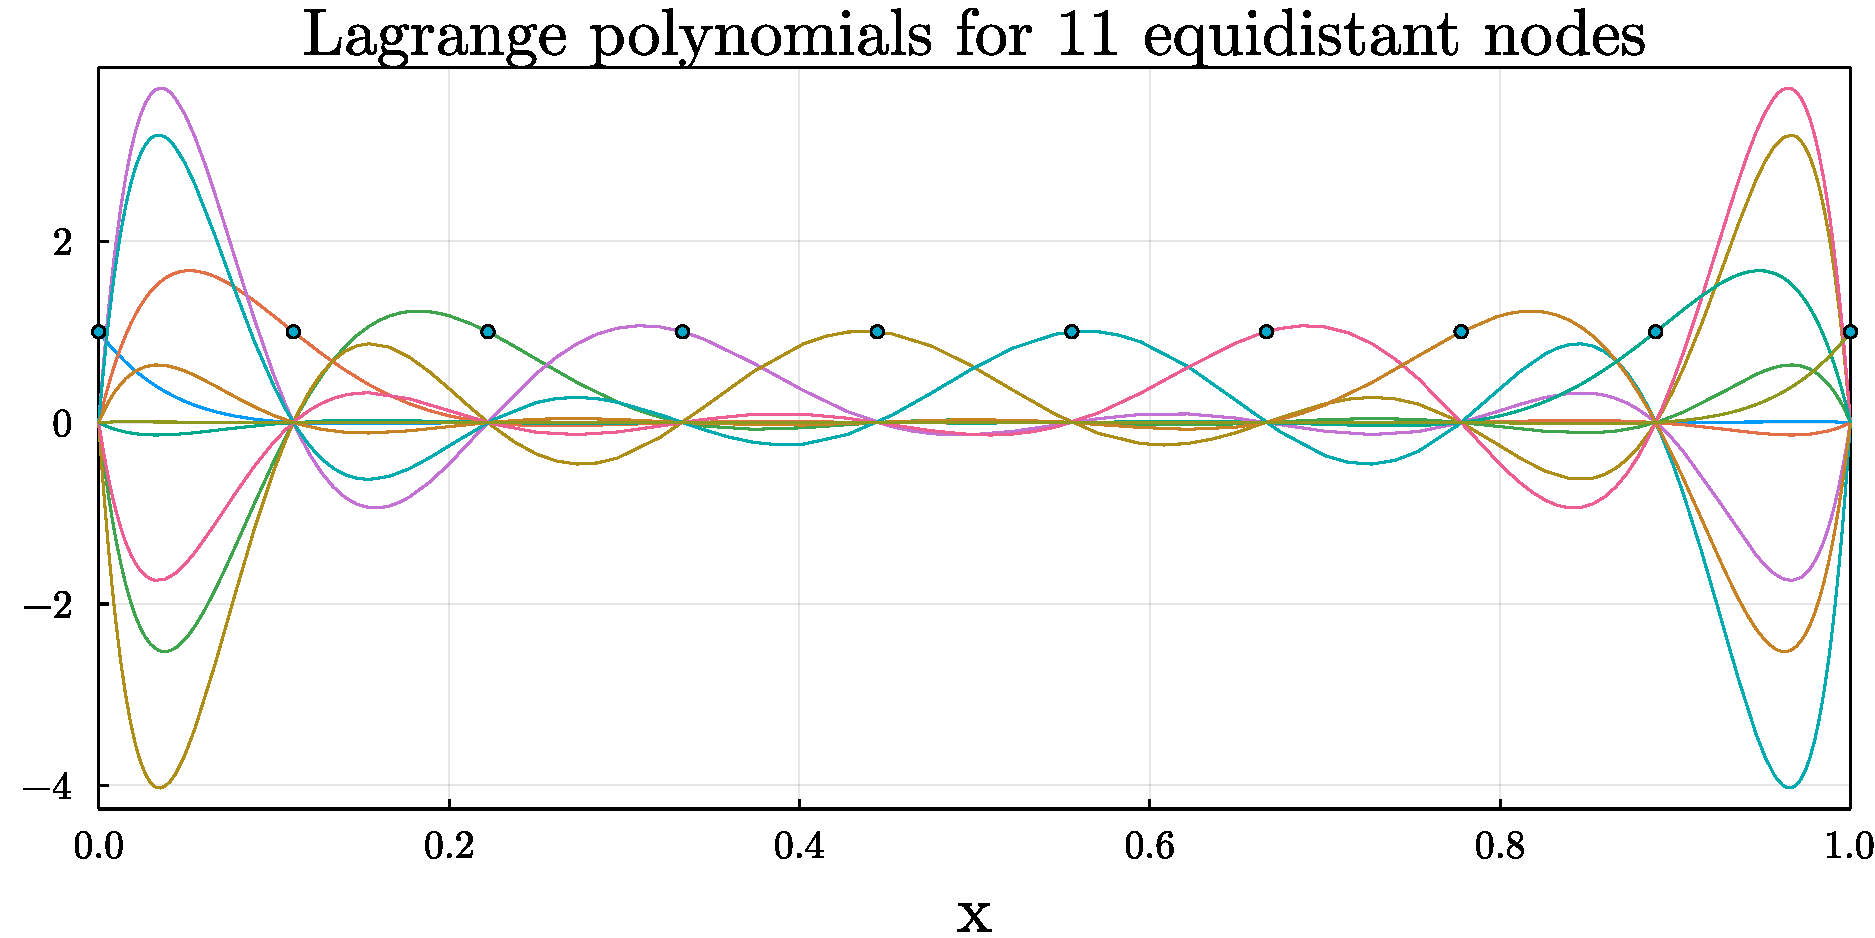
\includegraphics[width=0.8\linewidth]{figures/lagrange_10.pdf}
    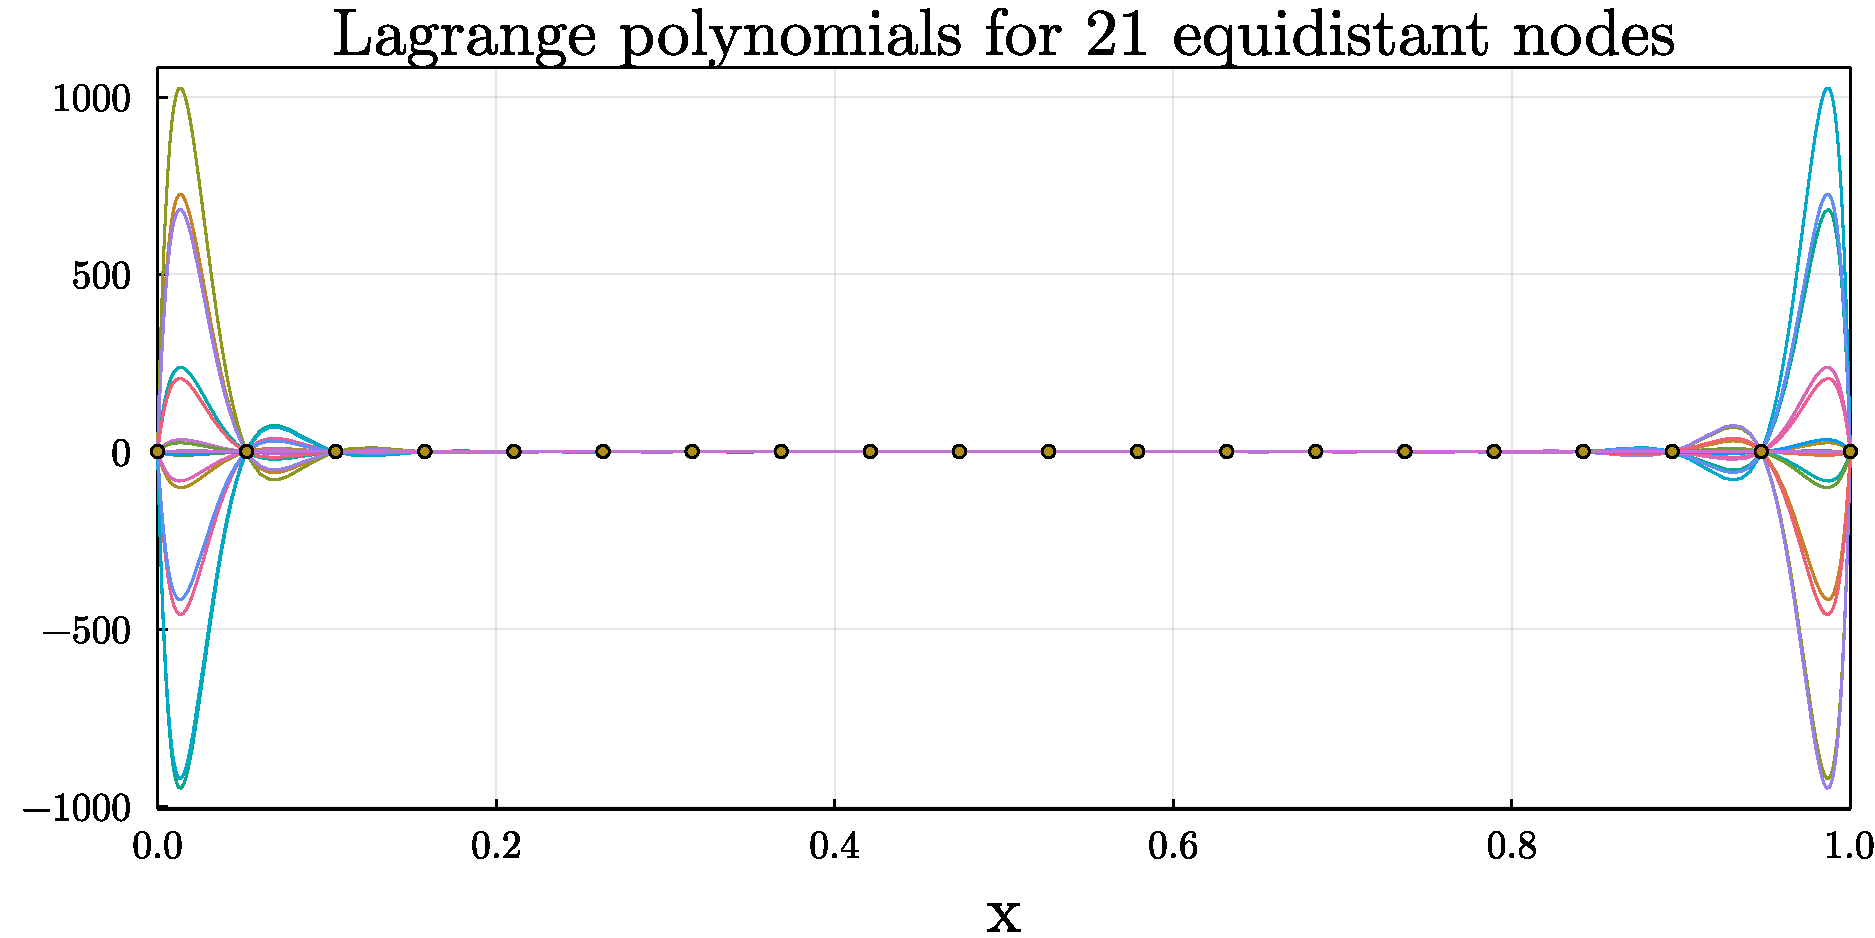
\includegraphics[width=0.8\linewidth]{figures/lagrange_20.pdf}
    \caption{Lagrange polynomials associated with equidistant nodes over the $(0, 1)$ interval.}%
    \label{fig:lagrange}
\end{figure}

\subsection{Gregory--Newton interpolation}
By Taylor's formula,
any polynomial~$p$ of degree $n$ may be expressed as
\begin{equation}
    \label{eq:taylor}
    p(x) = p(0) + p'(0) x + \frac{p''(0)}{2} x^2 + \dotsc + \frac{p^{(n)}(0)}{n!} x^n.
\end{equation}
In other words, the constant coefficient can be obtained by evaluating the polynomial at 0,
the linear coefficient can be identified by evaluating the first derivative at 0,
and so on.
Assume now that we are given the values taken by~$p$ when evaluated at the integer numbers $\{0, \dotsc, n\}$,
which we denote by $p_0, \dotsc, p_n$.
We ask the following question:
can we find a formula similar in spirit to~\eqref{eq:taylor},
but including only evaluations of $p$ and not of its derivatives?
To answer this question, we introduce the difference operator $\Delta$ which acts on functions as follows:
\[
    \Delta f(x) = f(x+1) - f(x).
    % (p_0, p_1, \dotsc) \mapsto (p_1 - p_0, p_2 - p_1, \dotsc).
\]
The operator~$\Delta$ is a linear operator on the space of continuous functions.
It maps constant functions to 0,
and the linear function~$x$ to the constant function~$1$,
suggesting a resemblance with the differentiation operator.
In order to further understand this connection,
let us define the \emph{falling power} of a real number $x$ as
\[
    x^{\underline{k}} = x (x-1) (x-2) \dots (x-k+1).
\]
We then have that
\begin{align*}
    \Delta x^{\underline{k}}
    &= (x+1) x (x-1) \dots (x-k+2) - x (x-1) (x-2) \dots (x-k+1) \\
    &= \bigl((x+1) - (x-k+1)\bigr) \bigl(x (x-1) \dots (x-k+2)\bigr) = k x^{\underline{k-1}}
\end{align*}
In other words,
the action of the difference operator on falling powers mirrors that of the differentiation operator on monomials.
The falling powers form a basis of the space of polynomials,
and so any polynomial in~$\poly(n)$, i.e.\ of degree less than or equal to $n$, can be expressed as
\begin{equation}
    \label{eq:gregory_newton}
    p(x) = \alpha_0 + \alpha_1 x^{\underline{1}} + \alpha_2 x^{\underline{1}} + \dotsb \alpha_n x^{\underline{n}}.
\end{equation}
It is immediate to show that $\alpha_i = \Delta^i p(0)$,
where $\Delta^i p$ denotes the function obtained after~$i$ applications of the operator~$\Delta$.
From the definition of~$\Delta$,
it is clear that the coefficients depend only on~$p_0, \dotsc, p_n$.
We conclude that, given points $n+1$ points $(i, p_i)$ for $i \in \{0, \dotsc, n\}$,
equation~\eqref{eq:gregory_newton} gives the corresponding interpolating polynomial.
An expansion of the form~\eqref{eq:gregory_newton} is called a \emph{Newton series},
the discrete analog of the continuous Taylor series.

\begin{example}
    \label{example:gregory_newton}
    Let us use~\eqref{eq:gregory_newton} to calculate the value of
    \[
        S(n) := \sum_{i=0}^{n} i^2.
    \]
    Since $\Delta S(n) = (n+1)^2$,
    which is a second degree polynomial in $n$,
    we deduce that $S(n)$ is a polynomial of degree 3.
    Let us now determine its coefficients.
    \begin{center}
    \begin{tabular}{|c|c|c|c|c|}
        \hline
        $n$    & $0$ & $1$ & $2$ & $3$ \\ \hline
        $\Delta^0 S(n)$ & $\mathbf{0}$ & $1$ & $5$ & $14$ \\ \hline
        $\Delta^1 S(n)$ & $\mathbf{1}$ & $4$ & $9$ &  \\ \hline
        $\Delta^2 S(n)$ & $\mathbf{3}$ & $5$ & & \\ \hline
        $\Delta^3 S(n)$ & $\mathbf{2}$ & & & \\ \hline
    \end{tabular}
    \end{center}
    We conclude that
    \[
        S(n) = \mathbf{1} n + \frac{\mathbf{3}}{2!} n(n-1) + \frac{\mathbf{2}}{3!} n(n-1)(n-2)
        = \frac{n (2n+1) (n+1)}{6}
    \]
\end{example}
Notice that when falling powers are employed as polynomial basis,
the matrix in~\eqref{eq:linear_system_interpolation} is lower triangular,
and the algorithm described in~\cref{example:gregory_newton} could be replaced by the forward substitution method.
Whereas the coefficients of the Lagrange interpolant can be obtained immediately from the values of~$u$ at the nodes,
calculating the coefficients of the expansion in~\eqref{eq:gregory_newton} requires $\mathcal O(n^2)$ operations.
However, this method has several advantages over Lagrange interpolation:
\begin{itemize}
    \item
        If a point~$(n+1, p_{n+1})$ is added to the set of interpolation points,
        only one additional term, corresponding to the falling power~$x^{\underline{n+1}}$,
        has to be calculated in~\eqref{eq:gregory_newton}.
        All the other coefficients are unchanged.
        Therefore, the Gregory--Newton approach is well-suited for incremental interpolation.

    \item
        The Gregory--Newton interpolation method method is more numerically stable than Lagrange interpolation,
        because none of the basis functions take very large values.
\end{itemize}
A polynomial in the form of a Newton series can be evaluated efficiently using Horner's method,
which is based on rewriting the polynomial as
\[
    p(x) = \alpha_0 + x \biggl( \alpha_1 + (x-1)  \Bigl( \alpha_2 + (x-2)\bigl(\alpha_3 + (x-3) \dotsc \bigr) \Bigr)  \biggr).
\]
Evaluating this expression starting from the innermost bracket leads to an algorithm with a cost scaling linearly with the degree of the polynomial.

\subsubsection*{Non-equidistant nodes}%
So far,
we have described the Gregory--Newton method in the simple setting where interpolation nodes are just a sequence of successive natural numbers.
The method can be generalized to the setting of nodes $x_0 \neq \dotsc \neq x_n$ which are not necessarily equidistant.
In this case, we take as basis the following functions instead of the falling powers:
\begin{equation}
    \label{eq:basis_newton}
    \varphi_{i}(x) = (x - x_0) (x - x_1) \dotsc (x - x_{i-1}),
\end{equation}
with the convention that the empty product is 1.
By~\eqref{eq:linear_system_interpolation},
the coefficients of the interpolating polynomial in this basis solve the following linear system:
\begin{equation}
    \label{eq:matrix_newton}
    \begin{pmatrix}
        1 &         & \ldots &        & 0  \\
        1 & x_1-x_0 &        &        &    \\
        1 & x_2-x_0 & (x_2-x_0)(x_2-x_1) &        & \vdots   \\
        \vdots & \vdots  &        & \ddots &    \\
        1 & x_n-x_0 & \ldots & \ldots & \prod_{j=0}^{n-1}(x_n - x_j)
    \end{pmatrix}
    \begin{pmatrix}
        \alpha_0 \\
        \alpha_1 \\
        \alpha_2 \\
        \vdots \\
        \alpha_n
    \end{pmatrix}
    =
    \begin{pmatrix}
        u_0 \\
        u_1 \\
        u_2 \\
        \vdots \\
        u_n
    \end{pmatrix}.
\end{equation}
This system could be solved using, for example, forward substitution.
Clearly $\alpha_0 = u_0$,
and then from the second line we obtain
\[
    \alpha_1 = \frac{u_1 - u_0}{x_1 - x_0} =: [u_0, u_1],
\]
which may be viewed as an approximation of the slope of~$u$ at $x_0$.
The right-hand side of this equation is an example of a \emph{divided difference}.
In general, these are defined recursively as follows:
\[
    [u_{0}, u_{2}, \dotsc, u_{d}] := \frac{[u_{1}, \dotsc, u_{d}] - [u_{0}, \dotsc, u_{d-1}]}{x_{d}-x_{0}}, \qquad [u_i] = u_i.
\]
It is possible to find an expression for the coefficients of the interpolating polynomials in terms of these divided differences.
\begin{proposition}
    Assume that $(x_0, u_0), \dotsc, (x_n, u_n)$ are $n+1$ points in the plane with distinct abcissae.
    Then the interpolating polynomial may be expressed as
    \[
        p(x) = \sum_{i=0}^{n} [u_0, \dotsc, u_n] \varphi_i(x),
    \]
    where $\varphi_i(x)$, for $i = 0, \dotsc, n$, are the basis functions defined in~\eqref{eq:basis_newton}.
\end{proposition}
\begin{proof}
    The statement is true for $n = 0$.
    Reasoning by induction, we assume that it holds true up to $n-1$.
    Observing $p(x) - u_0$ has a root at $x_0$,
    we deduce that
    \begin{equation}
        \label{eq:equation_newton}
        q(x) :=
        \frac{p(x) - u_0}{x - x_0}
    \end{equation}
    is a polynomial of degree at most $n-1$ that interpolates the points
    \begin{equation}
        \label{eq:newton_interpolation_vi}
        \left(x_i, v_i\right) := \left(x_i, \frac{u_i - u_0}{x_i - x_0}\right), \qquad i = 1, \dotsc, n.
    \end{equation}
    Using the induction hypothesis,
    we deduce that $q(x)$ is given by
    \[
        q(x) = \sum_{i=1}^{n} [v_1, \dotsc, v_i] (x-x_1) \dotsc (x - x_{i-1})
    \]
    By~\cref{exercise:divided_differences},
    it holds that
    \[
        [v_1, \dotsc, v_n] = \sum_{j=1}^{n} \frac{v_{j}}{\prod_{ k \in \{1, \dotsc, n\} \backslash \{ j\}} (x_{j} - x_{k})}.
    \]
    Employing the expression of~$v_j$ given in~\eqref{eq:newton_interpolation_vi},
    we have
    \begin{align*}
        [v_1, \dotsc, v_n]
        &= \sum_{j=1}^{n} \frac{\frac{u_{j}-u_0}{x_j - x_0}}{\prod_{ k \in \{1, \dotsc, n\} \backslash \{ j\}} (x_{j} - x_{k})}
        = \sum_{j=1}^{n} \frac{u_{j}-u_0}{\prod_{ k \in \{0, \dotsc, n\} \backslash \{ j\}} (x_{j} - x_{k})} \\
        &= \sum_{j=0}^{n} \frac{u_{j}-u_0}{\prod_{ k \in \{0, \dotsc, n\} \backslash \{ j\}} (x_{j} - x_{k})} = [w_0, \dotsc, w_n],
    \end{align*}
    where we introduced $w_i = u_i - u_0$, for $i = 0, \dotsc, n$.
    Now, since only differences appear in the divided difference $[w_0, \dotsc, w_n]$ and $w_i - w_j = u_i - u_j$ for all pairs $(i, j) \in \{0, \dotsc n\}^2$,
    it is clear that
    \[
        [w_0, \dotsc, w_n] = [u_0, \dotsc, u_n].
    \]
    Going back to~\eqref{eq:equation_newton} and rearranging,
    we conclude that
    \[
        p(x) = u_0 + (x-x_0) \left( \sum_{i=1}^{n} [u_0, \dotsc, u_n] (x-x_1) \dotsc (x - x_{i-1}) \right)
        =  \sum_{i=0}^{n} [u_0, \dotsc, u_{i}] \prod_{j=0}^{i-1} (x-x_j),
    \]
    which was the statement.
\end{proof}
\begin{example}
    Assume that we are looking for the third degree polynomial going through the points
    \[
        (-1, 10), \qquad (0, 4), \qquad (2, -2), \qquad (4, -40).
    \]
    We have to calculate $\alpha_i = [u_0, \dotsc, u_i]$ for $i \in \{0, 1, 2, 3\}$.
    It is convenient to use a table in order to calculate the divided differences:
    \begin{center}
    \begin{tabular}{|c|c|c|c|c|}
        \hline
        $i$ & $0$ & $1$ & $2$ & $3$ \\ \hline
        $[u_i]$ & $\mathbf{10}$ & $4$ & $-2$ & $-40$ \\ \hline
        $x_{i+1} - x_{i}$ & $1$ & $2$ & $2$ &  \\ \hline
        $[u_i, u_{i+1}]$ & $\mathbf{-6}$ & $-3$ & $-19$ &  \\ \hline
        $x_{i+2} - x_{i}$ & $3$ & $4$ &  &  \\ \hline
        $[u_i, u_{i+1}, u_{i+2}]$ & $\mathbf{1}$ & $-4$ & & \\ \hline
        $x_{i+3} - x_{i}$ & $5$  & &  &  \\ \hline
        $[u_i, u_{i+1}, u_{i+2}, u_{i+3}]$ & $\mathbf{-1}$ & & & \\ \hline
    \end{tabular}
    \end{center}
    We deduce that the expression of the interpolating polynomial is
    \[
        p(x)
        = \mathbf{10} + (\mathbf{-6})(x+1) + \mathbf{1} (x+1)x + (\mathbf{-1}) (x+1)x(x-2)
        = - x^3 + 2 x^2 + -3x + 4.
    \]
\end{example}

\section{Interpolation error}
Assume that~$u(x)$ is a smooth function and denote by $\widehat u(x)$ its interpolation through the points~$(x_i, u_i)$,
for $i = 0, \dotsc, n$.
In this section, we study the behavior of the error in the limit as $n \to \infty$.

\begin{theorem}
    [Interpolation error]
    Assume that~$u\colon [a, b] \to \real$ is a smooth function and let~$x_0, \dotsc, x_n$ denote $n+1$ distinct interpolation nodes.
    Then for all $x \in [a, b]$,
    there exists $\xi = \xi(x)$ such that
    \[
        e(x) := u(x) - \widehat u(x) = \frac{u^{(n+1)}(\xi)}{n+1!} (x-x_0) \dotsc (x - x_n).
    \]
\end{theorem}
\begin{proof}
    The statement is obvious if $x \in \{x_0, \dotsc, x_n\}$,
    so we assume from now on that $x$ does not coincide with an interpolation node.
    Let us use the compact notation $\omega_n = \prod_{i=0}^n (x - x_i)$ and introduce the function
    \begin{equation}
        \label{eq:interpolation_error}
        g(t) = e(t) \omega(x) - e(x) \omega(t).
    \end{equation}
    The function $g$ is smooth and takes the value~0 when evaluated at~$x_0, \dotsc, x_n, x$.
    Since $g$ has $n+2$ roots in the interval $[a, b]$,
    Rolle's theorem implies that $g'$ has $n+1$ distinct roots in~$(a, b)$.
    Another application of Rolle's theorem yields that $g''$ has $n$ distinct roots in~$(a, b)$.
    Iterating this reasoning, we deduce that $g^{(n+1)}$ has one root~$t_*$ in $(a, b)$.
    From~\eqref{eq:interpolation_error},
    we calculate that
    \begin{equation}
        \label{eq:interpolation_error}
        g^{(n+1)}(t) = e^{(n+1)}(t) \omega(x) - e(x) \omega^{(n+1)}(t)
        = u^{(n+1)}(t) \omega(x) - e(x) (n+1)!.
    \end{equation}
    Here we employed the fact that $\widehat u^{(n+1)}(t) = 0$,
    because $\widehat u$ is a polynomial of degree at most $n$.
    Evaluating~\eqref{eq:interpolation_error} at~$t_*$ and rearranging,
    we obtain that
    \[
        e(x) = \frac{u^{(n+1)}(t)}{(n+1)!} \omega(x),
    \]
    which completes the proof.
\end{proof}


\begin{exercise}
    \label{exercise:divided_differences}
    Show that
    \[
        [u_{0}, u_{1}, \dotsc, u_{n}] = \sum_{j=0}^{n} \frac{u_{j}}{\prod_{ k \in \{0, \dotsc, n\} \backslash \{ j\}} (x_{j} - x_{k})}.
    \]
\end{exercise}

\begin{exercise}
    using the Gregory--Newton formula,
    Find an expression for
    \[
        \sum_{i=1}^{n} i^4.
    \]
\end{exercise}

\begin{exercise}
    Using the Gregory--Newton formula,
    show that
    \begin{equation}
        \label{eq:discrete_exponential}
        \forall n \in \nat,
        \qquad 2^n = 1 + n + \frac{n^{\underline{2}}}{2!} + \frac{n^{\underline 3}}{3!} + \frac{n^{\underline 4}}{4!} + \dotsb
    \end{equation}
    \begin{remark}
        Remarkably, equation~\eqref{eq:discrete_exponential} holds in fact for \emph{any} $n \in \real_{> 0}$.
        However, showing this more general statement is beyond the scope of this course.
    \end{remark}
\end{exercise}
